\chapter{Results and Discussion}\label{chap_results}
% Within this section, your findings should be discussed with the aid of relevant graphs, figures or tables (with clear and concise captions). The information should be clearly presented and described in the text. You should make clear comparisons to relevant published studies and formulate answers to the research questions stated in your objectives section. Are your hypotheses supported by the findings?

% Discuss the advantages and disadvantages/limitations of methods used.

\section{Numerical Simulations}

%Preliminary study about the theory behind the Polymer Physics and the Physic of Turbulence was done. 
%After that the second step was regarding the Fortran code, in order to run the simulations is been necessary taking confidence and understand the code.
%Given the very complex structure of the code, read and understanding the more important \textsc{SUBROUTINE} of input and output.


%The code read all the variable parameter from a single file (\verb|rhea.i|), this file contains all the information regarding the operating condition and the initial-boundary condition, the order of interpolations that
%are computed during the iteration, the way to solve the algebric system. 


So far all the simulations performed had the same aims: to study the \textit{Polymer chain stretching phenomena}
considering a good solvent and a single polymer chain composed by 41 beads.

We want to understand in the Dilute polymer solution regime,
the mechanisms with which the polymer chain interact with turbulence eddies, in particular, figure out how the stretching process take places and how the polymer chain align with the eigenvectors of stress rate tensor.

We also want to find out a way to quantify the stretching. 

\subsection{Computational Grid Domain}

With a method so accurate like the Direct Numerical Simulation (DNS) the role of the grid becames fundamental, as detailed explain in sec.~\ref{sec:dns} there are certain parameters to be used in order to be sure that we are resolving all the turbulent length scales, and turbulent time scales. 

But it is also important that the \textit{aspect-ratio} of the cell is almost or equal to zero, so we discretize our domain with perfect cubic cells, and of course we have to use a 3D domain without any symmetry as shown in figure~\ref{mesh}. 


\begin{figure}[h]
\centering 
\includegraphics[width=.8\textwidth]{det.png}
\caption{detail of the cube computational grid}
\label{mesh}
\end{figure}
The whole domain is composed by a 3D box of dimension $0.6$x$0.6$x$0.6$ cm$^3$ in which all the surfaces have the periodic boundary condition discretized in 256 cell for edge (Total 16.777216e+6 cell).

Thanks to the periodicity we can consider homogeneous and isotropic turbulence. 



\newpage
\subsection{Initial Value, Parameters, and Boundary Condition}

In this subsection we will discuss the initial value and the value of the parameters used during ours simulations. 
In order to solve a system of Partial Differential Equation (Boundary Value Problem) , we need as many boundary conditions as the highest order in a space variable $x$ and $y$. If $u$ is the unknown, and the value of $u$ is given on the boundary then it is called Dirichlet's boundary condition(s).
If derivatives value are given they are called Neumann's boundary condition(s), and a Cauchy initial Value if the system of PDE is dynamic (initial value for the temporal variable, time).

To solve the problem it is also necessary to have the value of certain parameters.

\begin{table}[h]
\centering
\caption{Boundary, Parameter and Initial conditions}
\label{value}
\begin{tabular}{lc}
\toprule
\textbf{\color{blue}{Boundary/Parameter}} &\textbf{Value}  \\
\midrule
Surfaces & periodic bundary ccondition  \\
Initial Time & 0 \\ 
End Time &  $+\infty$ \\
$\Delta t$ & 5.5E-8\\
length of Edges ($l_{\small{\text{Box}}}$) &   0.6$cm$   \\ 
Node/Edge  & 256\\
Fluid Temperature  & 293.15 K\\
Interpoletion type & High ord. (6th) \\
$\rho$ (density) fluid & 0.9982 g/cm$^3$   \\
$\mu$ (Dinamic viscosity)  & 6E-5 cm$^2$/s  \\
$\nu$ (Kinematic viscosity)  & 6E-5/0.9982 g/(cm$\cdot$s) \\
CFL (Courant number)   & 0.6 \\
Hydrodinamic Interaction & Spectral \\
Turbulence               & Homogeneous Isotropic \\
Flow type               & Solenoidal  \\
Number of Chain          &     1  \\
Boltzman constant        & 1.38E-16 (g cm$^2$)/(s$^2$ K) \\
$\rho$ (density) solvent & 0.9982 g/cm$^3$        \\ 
solution $\theta$-Temp.  & 183.07 K \\
Polymer molar mass       & 1E+6 g/molecule    \\
Kuhn monomer molar mass  & 90.4977  \\
Kuhn monomer length      & 7.37E-8 cm \\
Random number generator  & 8 digit \\
Method for matrix sqr root & Cholesky/Chebyshev \\
Brownian motion           & On \\   
\bottomrule
\end{tabular}
\end{table}


In order to avoid wrong results physically, checking that the turbulence parameters are correct with respect to the 
grid sizes was necessary (they contain the entire polymer chain) it is suitable respect the \textit{Direct Numerical Simulation}
required parameters (max dimensions respect to the Reynolds number). 

\subsubsection{Kolmogorov Length scale}

The \textit{Kolmogorov} length scale is given by the Eq.~\ref{eq:kscale},
we know the value of $\nu$ (scaled from the file \verb|memo.dat|, unscaled from \verb|rhea.i|), we also know the scaled value of $\epsilon$ from the output of the code (file \verb|snf_quad.dat|). We can thus compute the Kolmogorov length scale in two different ways:
\begin{enumerate}

\item \textbf{Unscaling} $\mathbf\epsilon$ using its scaling factor:
$$\epsilon \sim \frac{UU}{L/U} \sim \frac{U^3}{L} $$
since we know the scaling factor of the velocity $U$ and the length $L$

\item Using the scaled value of $\nu$ and computing the scaled value of the lenght scale $\eta$ and then multiply this for the time scaled factor (obtained from \verb|memo.dat|)  

\end{enumerate}

Using the method 1, and the method 2 we obtain the same result. 
The known values are reported in the table~\ref{value} :

\begin{table}[h]
\centering
\caption{Known Values}
\label{value}
\begin{tabular}{ccc}
\hline
\textbf{Quantities} &scaled value  &unscaled value  \\
\hline
$\nu$ & 39420.23  &  1.E-2/0.9982 $cm^2/s$    \\
$\epsilon $ &0.2068E-3  & -     \\
$U$                 &0.87   & - \\
$L$             & 7.370E-008 & 0.6 cm \\
$time$          & 2.1373E-008 & 0.295 s \\ 
\end{tabular}
\end{table}


We report just the Method 1 here: (Unscale $\epsilon$)

The scaling factor of $\epsilon$ is proportional to $U^3/L$ we know 
the scaling factor of U and L as reported in Table~\ref{value} 

Therefore we can calculate the scalar factor for $\epsilon$
\begin{equation}
\epsilon = \tilde{\epsilon}  \frac{U^3}{L}  =  0.2068E-3   \frac{0.87^3}{7.370E-008} = 0.2068E-3 \frac{0.658503}{7.370E-008} = 1847.95 
\end{equation} 

now using the unscaled value of $\epsilon$ we can calculate 
the value of $\eta$ given from the equation: 

\begin{equation}
\eta = \left( \frac{\nu^3}{\epsilon} \right) ^{1/4} =  
\left( \frac{(1.0E-2/0.9982)^3}{1847.95} \right) ^{1/4} = (5.44352E-10)^{1/4} = \mathbf{0.0048296}
\end{equation}

The cell size is given by L$_\text{box}$/N$_{\text{cell}}$ for edge = 0.6 / 256 = \textbf{0.002343}.

Therefore the smaller eddies stay in the cell : $0.0048296/0.002343 = 2.16$ (almost two times). Hence the size is correct, with respect to the condition given in the Eq.~\ref{cond1}. 

\subsubsection{Time scales}
The time of large eddy turn over is defined by 
\begin{equation}
t_L = \frac{L}{U} 
\end{equation}

As reported in Table~\ref{value} we know the Length of the computational domain (0.6cm) the velocity $u$ and its scalar factor, so it is easy to calculate the Time of large eddy turn over:
$$U = \sqrt{\overline{u}} \cdot \tilde{u} \qquad  \qquad L = L_{\text{Domain}}/2 $$
where with $\tilde{u}$ means the velocity scalar factor and $\overline{u}$ the velocity calculated by the code, the Large Eddy turnover is therefore:
\begin{equation}
t_L = \frac{0.6/2}{6.8454} = \mathbf{0.043825} 
\end{equation}
This means that the simulation must run for not less than this time, in order to catch all the phenomena. 

\subsubsection{Kolmogorov Time Scale}
We can also compute a time scale for the small eddies using viscosity and dissipation rate~\ref{eq:timeeta}.

%\begin{equation}
%t_{\eta} = \left( \frac{\nu}{\epsilon} \right)^{1/2} 
%\end{equation}

This can be calculated using $\epsilon$ scaled and $\nu$ scaled and then multiplying the result for the time-scaled factor.

\[
\tilde{t_{\eta}} = \left( \frac{\nu}{\epsilon} \right)^{1/2} = \left( \frac{39420.23}{0.2068E−3} \right)^{1/2} = 190620067.698^{1/2} = 13799.85
\]

now using the time unscaling factor :
\[t_{\eta} = \tilde{t_{\eta}} \cdot K_T = 13799.85 \cdot 2.1373E-008 = \mathbf{0.000295}\]

where $K_T$ is the time scale factor.
%\newpage
\section{Polymer chain consideration}

For a polymer chain, as it is known, the brownian motion of the monomers could be described as an random motion  for effect of the solution temperature, so we modelled it using a 8-digit random number generator. 


\begin{figure}[h!]
\centering
\includegraphics[width=.82\textwidth]{pol_length.pdf}

\caption{Polymer chain in a turbulent flow - Stretching phenomena}
\label{polength}
\end{figure}

It is possible to observe in Fig.~\ref{polength} how this motion affects slighly the polymer length (the oscillation with respect to the time).
From the same figure we can also notice that after a certain period of time the polymer length increases almost istantanely, after that, the length decreases a bit slowly respect to the previous increase (relaxation), this is the tipical behaviour of the polymer stretching, that in this case takes place after $0.002925 s$ (24000 time-step of simulation).
Now we have observed only one strecthing event for simulation, using different digit of the random number generator the starting point of stretch slighly changes, as is shown in Fig.~\ref{rand}, in wich there is five simulation in running.   

\begin{figure}[h!]
\centering
\includegraphics[width=.95\textwidth]{polengthRand.pdf}
\caption{Simulations with different seed number for random generator}
\label{rand}
\end{figure}

Using different digit to generate the random fluctuation (brownian motion of the chain) the polymer is still confined around its initial position, so as we can observe from the Fig.~\ref{rand} the stretch takes place 
almost after the same period of time (arount 0.003$s$). This behaviour is due to the fact that the turbulent eddies in a homogeneous and isotropic turbulence are basically random too, and starting from the same boundary condition, thus the flow field situation that causes the stretch of the chain, takes place in the position in which the polymer is confined, take place after the same period of time. %this is the reason for which the streach tache place around the same period of time. 

\begin{figure}[h!]
\centering
\includegraphics[width=.8\textwidth]{XY}
\caption{xy plane}
\label{xy}
\end{figure}
Hence if we want to observe several stretching phenomena we have to modify the initial position of the chain 
with respect to the box. 
In order to do this we have to modify the random parameter that generate the initial position of the polymer configuration with respect to the box. This parameter generate the sequence of monomers starting from the initial point (first monomer) randomly placed inside the box.

To observe the behaviour of chains confined in different initial positions we run three simulations using different random number for the polymer sequence configuration on the 3D computational domain. 

As reported in Fig.~\ref{xy}, in which the plane $xy$ is rapresented, we can observe the three different initial positions rapresented from the markers (red, blue and black) inside the turbulent flow fied. 
These simulations are still in running and so far no stretch event was not observed.

\subsection{Stretching Phenomena consideration}
\begin{figure}[h!]
\centering
\includegraphics[width=.82\textwidth]{pol_dl.pdf}
\caption{Detail of the peak, Stretching phenomena}
\label{detail}
\end{figure}

Considering the detailed of the stretch event reported in Fig.~\ref{detail}, the picture represents the starting 
point in which the chain became stretched almost istantanelly, and its return to the relaxed dimension.



\begin{figure}[h!]
\centering
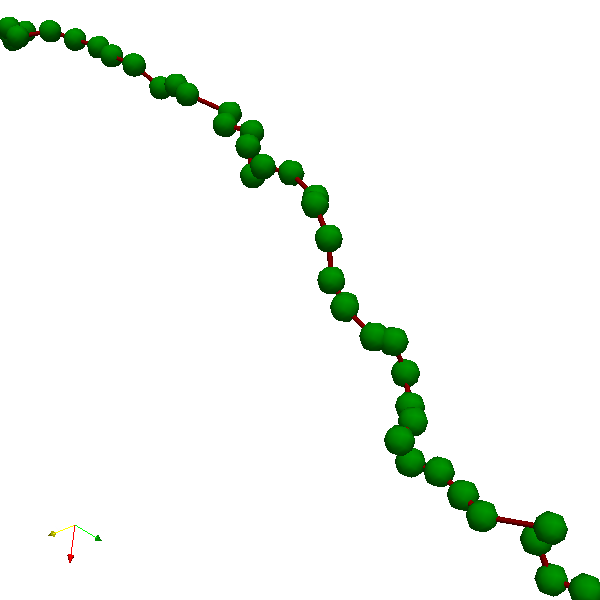
\includegraphics[width=.52\textwidth]{poly-stretch}
\caption{Polymer under stretching phenomena}
\label{detail}
\end{figure}

Since the polymer chain is smaller then a single cell, a vortex able to interact with the chain should be approximately of the dimension of one cell. This can be verified observing the duration of the event reported in the picture with the ``L'' label that is around 0.00022$s$. 
If we compare the time of the event with the time scale for the smallest eddies (0.000295$s$) we can deduce that a smallest eddy caused the stretching of the chain after that the eddy disappears, the time of duration of this event is infact the ``life-time'' of the small eddies.








%\begin{figure}[tb]
%\centering
%\hspace{-0.5in}
%\subfloat[x=0.0m]
%{\label{av-x0-dev-coarse}
%\includegraphics[width=.5\columnwidth]{immagini/coarse/dev-edm/x000-axialvel.pdf}}
%\subfloat[x=0.25m ]
%{\label{av-x025-dev-coarse}
%\includegraphics[width=.5\columnwidth]{immagini/coarse/dev-edm/x025-axialvel.pdf}} \\
%\hspace{-0.5in}
%%\vspace*{1.7in}
%\label{av-x05-dev-coarse}
%\subfloat[x=0.5m]
%{\includegraphics[width=.5\columnwidth]{immagini/coarse/dev-edm/x050-axialvel.pdf}}  %, trim=0 4cm 7cm 0,clip
%\subfloat[x=0.85m]
%{\label{av-x085-dev-coarse}
%\includegraphics[width=.5\columnwidth]{immagini/coarse/dev-edm/x085-axialvel.pdf}}\\
%\caption{\label{edm-dev-axvel}Velocità Assiale, confronto modelli di devolatilizzazione EDM}
%\end{figure}
%
